\documentclass[a4paper,10pt]{book}
\usepackage[utf8]{inputenc}

\usepackage[utf8]{inputenc}
\usepackage[english]{babel} %francais, polish, spanish, ...
\usepackage[T1]{fontenc}


\usepackage{amsfonts}
\usepackage{amsmath}
\usepackage{amssymb}
\usepackage{graphicx}
\usepackage{dcolumn}
\usepackage{latexsym}
\usepackage{hyperref}
\usepackage{bm}
\usepackage[english]{babel}
\usepackage{xcolor}



\usepackage{lmodern} %Type1-font for non-english texts and characters
\usepackage{amsthm}
\usepackage{amsfonts}
\usepackage{float}
\usepackage{ mathrsfs }


\usepackage[utf8]{inputenc}
\usepackage[T1]{fontenc}
\usepackage{textcomp}
\usepackage{gensymb}
\usepackage{subcaption}

\def \ep{\epsilon}

\newtheorem{lemma}{Lema}
\newtheorem{ejemplo}{Ejemplo}
\newtheorem{definition}{Definción}
\newtheorem{theorem}{Teorema}

\begin{document}


\section{Introducci\'on}
Queremos buscar los m\'inimos del siguiente problema:$\mathscr{L}$ es un operador lineal
$\mathscr{L} u=f$.   Si definimos
\[A(u,v)=\iint_{\Omega} \mathscr{L} u v  dx dy \] 
donde $dx dy$ representar\'a un diferencial de area y en general lo omitiremos.
$A$ es tal que $A(u,v)\geq \alpha {|| u ||}^2$ si  $u_0$ es m\'inimo de 
\[A(u,u)-2 (f,u) \]
donde se define
\[(f,u)=\iint_{\Omega} f u .\]
entonces a $u_0$ se le llama la soluci\'on generalizada de $\mathscr{L} u=f$. El operador $\mathscr{L}$ puede ser 
por ejemplo la  biarm\'onica $\Delta^2$.
si
\[\iint_{\Omega} \mathscr{L} u\phi =\iint_{\Omega} f \phi  \]
para todo $\phi \in C_0^\infty$, entonces definimos el operador autoadjunto como 
\[\iint_{\Omega} \mathscr{L}^{*} u\phi \]
donde $*$ indica complejo conjugado. Ejemplos f\'isicos de este operador son 
la membrana el\'astica y el campo electrost\'atico. En cualquiera de estos casos
vemos que la energ\'ia almacenada por el campo se puede escribir de la forma
\[I(u)=\iint_{\Omega} |\nabla u |^2  .\]
El problema lo plantearemos como : encontrar $u$  que minimiza $I(u)$ con $u|_{\partial \Omega}=f$ .
Primero veremos que el minimizar la energia es equivalente a encontrar la soluci\'on al problema 
del laplaciano con valor en la frontera. Sea $v$ tal que $v|_{\partial \Omega}=f$ y sea
$h=v-u$ entonces $h|_{\partial \Omega}=0$. Ahora
\[I(v)= I(u+h)=  \iint_{\Omega} (u_x +h_x)^2+(u_y+h_y)^2  \]
donde si utilizamos una de las identidades de Green que se sigue del teorema de la divergencia con 
el campo vectorial $u \nabla v $ y usando el hecho que $\partial_{k}(u\partial_k v)=u \partial _k \partial _k v+  \partial _k u \partial _k v$,
donde se asume  suma sobre indices repetidos, entonces

\[\iint_{\Omega} \nabla \cdot (u \nabla v)   =\iint u \Delta v + \iint_\Omega \nabla u\cdot\nabla v \]
donde  aplicandolo a la energ'ia y recordando que $h$ vale cero en la frontera encontramos que

\[I(v)=I(u)+I(h)-2\iint_{\Omega} h \Delta u  \] 
donde usamos el hecho que $h$ vale cero en la frontera. Si el laplaciano de $u$ es positivo en un punto $(x_0,y_0)$
entonces ser\'a positivo en una vecindad de $(x_0,y_0)$.  Tomamos $h<0$ en la vecindad de $(x_0,y_0)$
fuera de dicha vecindad, entonces se tiene que $I(u+h)\geq I(u)$. Ahora si tomamos
$h>0$ en la vecindad y cero fuera y tal que $\iint_{\Omega} |\nabla h|^2 =1$   entonces
\[I(u+\epsilon h)-I(u)= \epsilon^2-2\epsilon \iint_{\Omega} h \Delta u <0\]
si $ \epsilon$ es peque\~no, lo que contradice que $I(u)$ sea m\'inimo. Lo que implica que
$\Delta u\leq 0$ y por lo tanto $\Delta u=0$ y por lo tanto $u$ m\'inimo de $I(u)$  con $u|_{\partial \Omega} =f$ es necesario
y suficiente para que $\Delta u=0$ en $\Omega$ y $u|_{\partial \Omega}=f$.

\subsection*{\underline{La soluci\'on es \'unica}.}

Si $u_1$ y $u_2$ son soluciones, $h=u_1-u_2$ entonces
\[I(u_1)=I(u_2+h)=I(u_2)+I(h)\]
y como $I(u_1)=I(u_2)$ implica que $I(h)=0$ y por lo tanto $\nabla h=0$ y por lo tanto 
$h=cte=0$ en $\partial \Omega$.

\subsection*{\underline{Principio de Dirichlet}.}
Tenemos las siguientes preguntas:
\begin{enumerate}
 \item \textquestiondown Existe una soluci\'on de $\Delta u=0$ 
en $\Omega$, talque $u|_{\partial \Omega}=f$ ?.\textquestiondown Que tipo de solución es ?
Acaso $u\in C^2 (\Omega) \cap C^0 (\bar{\Omega})$ donde la barra indica la cerradura de $\Omega$.
Si es \'unica  $h=u_1-u_2$ implica $\Delta h=0$ y $h|_{\partial \Omega} =0$ implica el principio
del m\'aximo que a su vez implica que $h=0$.

\item \textquestiondown Existe un m\'inimo ?
\item \textquestiondown Como se calcula el m\'inimo $I(u)=\iint_{\Omega}  |\nabla u|^2 $.
\item Si existe el m\'inimo $u$ implica acaso que $u\in C^2 (\Omega) \cap C^0 (\bar{\Omega})$ implica 
acaso que la energ\'ia es finita ?
\end{enumerate}

Ilustraremos estas preguntas con un ejemplo. 

\subsection*{1)\underline{Ejemplo de Hadamard}.}

Sea $\Omega $ un disco unitario. Consideremos la funci\'on sobre la frontera del 
disco unitario parametrizada por el \'angulo $\theta\in [0,2\pi]$

\begin{equation}
\label{hadamard}
  f(\theta)=\sum\limits_{n=1}^{\infty} \frac{cos(2^{2n} \theta)}{2^n}
\end{equation}

Como $|f(\theta)|\leq \sum\limits \frac{1}{2^n} =1$ (como puede verse de sumar la serie geom\'etrica con $r=1/2$),
entonces al serie es absolutamente convergente. Que implica que $f(\theta)$ es continua.
sea 
\[u(x,y)=u(\rho,\theta)=\sum\limits_{n=1}^{\infty}  \rho ^{2 ^{2n} } \frac{\cos(2^{2n} \theta)}{2^n}\]
esta funci\'on cumple que $u|_{\partial \Omega}=f(\theta)$  y $|u(x,y)|\leq 1$ y
\[u(x,y)= Re \left( \sum\limits_{n=1}^\infty \frac{z^{2^{n}} }{2^n}\right) \]
es una funci\'on anal\'itica para $|z|<1$  lo que implica que $u$ es arm\'onica. Ahora para pasar a coordenadas
polares usamos el hecho que 
\[u_x=u_\rho \cos \theta - u_{\theta} \frac{\sin \theta}{\rho} \]
\[u_y=u_\rho \sin \theta  + u_{\theta} \frac{\cos \theta}{\rho}.\]

La energ\'ia se calcula como
\[ I(u)= \iint_{\Omega} (u_x^2+u_y^2)= \int_0^1 \int_0^{2\pi} \left( u_{\rho} ^{2} + \frac{u_\theta ^2 }{\rho^2} \right) \rho d\rho d\theta
\]
Sustituyendo se tendr\'ia que

\[ I(u)= \int_0^1 \int_0^{2\pi} \left( 
 \sum\limits_{n=1}^{\infty}  2^{2n} \frac{\rho ^{2 ^{2n}-1 } }{2^n} \frac{\cos(2^{2n} \theta)}{2^n} \right)^2+
\]
\[
 \left( 
 \sum\limits_{n=1}^{\infty} (-) 2^{2n} \frac{\rho ^{2 ^{2n} } }{2^n} \frac{\sin(2^{2n} \theta)}{2^n} \right)^2 \frac{1}{\rho^2} \rho 
d\rho d\theta.
\]

Como los dobles productos de senos y cosenos son cero, entonces

\[I(u)=\left.2\pi \sum\limits_{n=1}^{\infty} \frac{2^{2n}}{2^{2n+1} } \rho^{2^{2n+1}}\right|_0^1=\pi \sum\limits_{n=1}^{\infty} \rho^{2n+1}=\infty.\]

Moraleja, tengo que trabajar con una clase m\'as chica de funciones en la frontera. Esta clase ser\'a $f|_{\partial \Omega}$ y
si definimos los siguientes espacios, entonces

\[ L^2 (S^1)=\left\lbrace g(\theta)=\sum\limits_{n=-\infty}^{\infty} a_n e^{i n \theta } \in Re \Leftrightarrow
 a_{-n}=\bar{a}_n \right\rbrace
\]
con 
\[\sum\limits |a_n|^2 =\int_{0}^{2\pi} |g(\theta)|^2 d\theta < \infty \]

Podemos definir los espacios de funciones
\[H^{\alpha}(S^1)=\left\lbrace  g(\theta) = \sum\limits_{-\infty}^{\infty} a_n e^{in\theta}, a_{-n}=\bar{a}_n, \sum\limits_{-\infty}^{\infty} |a_n|^2 n^{2\alpha} <\infty  \right\rbrace.
\]
en particular
\[H^1(S^1)=\left\lbrace g: \sum\limits_{n=-\infty}^{\infty} | a_n|^2 n^2 =\int_0^{2\pi} |g'(\theta)|^2 d\theta \right\rbrace < \infty \] 
Para ver a que espacio de funciones corresponde la funci\'on  del ejemplo de Hadamard (\ref{hadamard}) vemos que
\[\sum\limits_{-\infty}^{\infty} |a_n|^2 n^{2\alpha} =\sum\limits_{n=-\infty}^{\infty} \left(\frac{1}{2^n} \right)^2 (2^{2n} )^{2\alpha} =\sum\limits_{n=-\infty}^{\infty} \frac{1}{2^{2n(1-2\alpha)}} \] 
que ser\'a menor que infinito si $\alpha <1/2$  y la serie converge uniformenente. Si $\alpha\geq 1/2$ tenemos una
suma infinita y por lo tanto $f(\theta)\in H^{\alpha}(S^{1} )$ con $\alpha<1/2$ .
Se puede probar que si $f(\theta)\in H^{\alpha}(S^1)$, $\alpha\geq 1/2$ entonces existe
$u$ tal que $u|_{\rho =1}=f$ y $I(u)<\infty$ . (teorema de traza, adem\'as $f$ es continua)

\subsection*{2)\underline{Tipo de soluciones}.}

Sea $f|_{\partial \Omega}$ tal que exista $u_0 \in C^2(\Omega) \cap  C^0(\bar{\Omega}) $, $u_0|_{\partial \Omega}=1$ y $I(u_0)< \infty$.
Sea $u$ talque $\nabla^2 u=0$ , $u\in C^2(\Omega)\cap C^0(\bar{\Omega})$, $I(u)<\infty$, $u|_{\partial \Omega}=f$ sea 
$h=u-u_0$ implica $h \in C^2(\Omega) \cap  C^0(\bar{\Omega})$, $\Delta h=\Delta u-\Delta u_0=-\Delta u_0=g$  es continua. 

Sea 
\[J(k)=\iint_\Omega| \nabla k|^2  + 2\iint_\Omega gk \]
para $k\in C^2 (\Omega)\cap C^0(\bar{\Omega}) $, $k|_{\partial \Omega}=0$ , $I(k)<\infty$. Si definimos

\[J(h)=I(h)+2 \iint_\Omega \Delta h h  = I(h) -2\iint_\Omega | \nabla h |^2 = -I(h)\]
donde hemos utilizado la identidad de Green. Ahora 
\[J(h+k)= I(h+k)+2\iint (h+k)g  \]
\[J(h+k)= I(h)+I(k) -2 \iint k \Delta h+2\iint  (h+k)g \]
\[J(h+k)=J(h) +I(k)+2 \iint_\Omega( g-\Delta h )k \]
cuando $g-\Delta h =0$ da el m\'inimo  de $J(k)$. Alrev\'es,  si $h$ tiene esas propiedades y $J(h)$ es
m\'inimo entonces $\Delta h=g$ en $\Omega$. Entonces tenemos que si definimos el espacio de funciones
\[E=\left\lbrace k\in C^2 (\Omega) \cap C^0(\bar{\Omega} ), k|_{\partial \Omega}=0 \right\rbrace, I(k)<\infty\]
entonces $  \underset{E}{min} J(k)$  es una condici\'on necesaria y suficiente para que $h$ 
sea soluci\'on de la ecuaci\'on si $\Delta h=g$ y como se vi\'o se tiene que

\begin{enumerate}
\item $J(h)=-I(h)$
\item $J(h+k)= J(k)+I(k)$
\item $J(k)\geq I(k)-2\iint_\Omega |g||k| \geq I(k) - \epsilon \iint_\Omega k^2 -\frac{1}{\epsilon} \iint_\Omega g^2 $ \\
donde en $3)$ se utiliz\'o el hecho que si $a,b$ son dos n\'umeros cualesquiera entonces siempre se tiene
que  $2ab\leq \epsilon a^2 +\frac{1}{\epsilon} b^2 $ (teorema del binomio) . Si $|k|=0$ en $\partial\Omega$ entonces el lema de Poincar\'e
nos da que 
\[ \iint_\Omega k^2 \leq \kappa \iint_\Omega |\nabla k|^2\]
donde tomando  $\epsilon=1/\kappa$ tenemos que
\[J(k)\geq -\kappa \iint_\Omega g^2 \]
es decir $J$ es acotado por abajo.

\item Si existe el minimo $k\in E$ ¿aproxima a $h$?

sean $w_1,w_2,....\in E$. "linealmente independientes", tal que cualquier $K$ en $E$ 
es "aproximado" por una combinación finita de las $w$'s
si $\Delta h = g$ y $h|_{\partial \Omega} = 0$

Sean $E_N= \{ \sum\limits_{1}{N} a_i w_i \}$ tiene dimension $N$ $E_N \rightarrow\{ a_1,...,a_N\}$

\[
J_N(a_1,...,a_n) = J |_{E_N} = \iint |\nabla \sum\limits a_i w_i |^2 + 2g \sum\limits a_i w_i 
\]
\[= \iint \sum\limits_{i,j =1}^N a_i a_j \nabla w_i\cdot w_j + 2 \sum\limits_{i}^N a_i g w_i = \text{ polinomio de grado 2 en } a_1,...a_n\]
\[
J_N\geq -k \iint g^2  \Rightarrow \text{ hay un mínimo}
\]

dado por $\frac{\partial J_N }{\partial a_i} = 0$

\[
\frac{\partial J_N }{\partial a_i} = 2 \iint \left(  \sum\limits_{j=1}^M a_j \nabla w_i \cdot \nabla w_j + g w_i \right) = 0 \;\; i=1,...,N
\]

Sea  $ A_N= \left( \iint_{\Omega} \nabla w_i \cdot \nabla w_j \right)_{ij}$  $B_n= -\left(\iint g w_i  \right)_i $
\[
A_N  \left( 
\begin{array}{c} 
a_1\\
\vdots\\
a_n
\end{array} 
\right)=B_N  \;\;\;\; \text{ linealmente independiente } \Leftrightarrow  A_N \text{ invertible } \forall N
\]

\[
\Rightarrow 
\left( 
\begin{array}{c} 
a_1\\
\vdots\\
a_n
\end{array} \right) = A_N ^{-1} B_N 
\]
  única solución, mínimo de $J_N$
$U_N = \sum\limits_1^{N} a_i w_i$  $J(U_N)= J_N$ es mínimo sobre $E_N$

$A_N= A_N^{T}$

¿$J_N \rightarrow J(h) $?

¿$U_N \rightarrow h$?

en que sentido

$J_N$ $ E_N \subset E_{N+1}$  $J_N \geq J_{N+1} \Rightarrow \{J_N\}\downarrow $ y acotado por abajo entonces
$J_N\rightarrow d$.

Supongamos que si $k\in E \Rightarrow $ existe $v_N \in E_N$ con $I(v_N -k) \rightarrow 0$,  $(v_N\rightarrow k )$ en $H^1$

$h\in E \Rightarrow $ existe $v_N \in E_N $ con $I(v_N-h )\rightarrow 0$

\[
\begin{array}{ccc}
     J(h) & \leq J(U_N)  & \leq J(v_N-h+h)  \\
      \shortparallel &  & \\
      \text{mínimo sobre } E& & = J(h) +I ( v_N-h)  \rightarrow 0
\end{array}
\]

$E_n \Rightarrow J(U_N), \; J(v_N) \rightarrow J(h)$ 

\[
\begin{array}{cc}
I(U_N-k)  & \text{si}  U_N-k = U_N -k +h - h \\
\shortparallel &   \\
J(U_n-k+h) -J(h) &= J(U_N)-J(h) \rightarrow 0
\end{array}
\]

\[
\iint |\nabla ( U_N -h ) | ^2 dx  \overset{N\rightarrow \infty}{ \rightarrow 0} \;\;\; \text{aproximación de $h$ por $U_N$ en el sentido $H^1$}
\]

¿Espacio de trabajo?   $ k \in C^2 (\Omega) \cap  C^0 (\bar{\Omega}) \overset{\Delta}{\rightarrow} C^0(\Omega)$


\begin{ejemplo}
    $\Omega = \{x \in \mathbb{R}^3  : |x|<1  \}$

\[
    \begin{array}{c}
         \Delta h= g  \\
         h|_{\partial \Omega }=0  
    \end{array} \Rightarrow 
\]
 \[
   h(x) = -\frac{1}{4\pi} \iiint_{|\xi|<1 } \frac{g(\xi)}{ |x-\xi|} d\xi  + \frac{1}{4\pi} \iiint_{|\xi|<1 } \frac{g(\xi)}{ |\frac{x}{|x|^2}-\xi|}   d\xi
\]
El segundo término es $C^\infty$, el primero lo vamos a analizar en un caso especial.

    Sea 
\[
 g(x)  = \left\{\begin{aligned}
        \left(  \frac{3 z^2}{ |x|^2} -1\right) \frac{1}{log \frac{|x|}{2} }  & \text{ si } x\neq 0 \;\; C^\infty\\
        0 & \text{ si } x = 0,
       \end{aligned}
 \right.
\]

$g(x)$ es continua en $\Bar{\Omega}$

si $x\rightarrow 0 $. $ 0\leq \frac{3 z ^2}{|x|^2 }\leq 3 $

entonces

\[
-\frac{1}{4\pi} \iiint_{|\xi|<1 } \frac{g(\xi)}{ |x-\xi|} d\xi  =  -\frac{1}{4\pi} \int_0^{2\pi}\int_0^{\pi}\int_0^1 (3\cos\theta^2-1) \frac{1}{\log \frac{r}{2}} \frac{r^2}{|x-\xi| } \sin \theta dr d\theta d\phi
\]


\[
I_1 =  -\frac{1}{4\pi} \int_0^{2\pi}\int_0^{\pi}\int_0^1 \frac{(3\cos\theta^2-1)\sin \theta r^2 }{ \left(r^2 +a^2 -2 a r \cos{\theta} \right)^{1/2} \log \frac{r}{2}}  dr d\theta d\phi
\]

para evaluar la integral orientamos $x = (0,0,a)$ a lo largo del eje $z$ y el cambio de variable

$t^2 = r^2 +a^2 -2 a r \cos{\theta}$

$2t dt = 2 a r \sin{\theta} d\theta$

\[
I_1= - \frac{1}{2} \int_0^1 \int_{|r-a|}^{r+a} \left(  3 \frac{(t^2 - r^2 -a^2)^2}{(2ar)^2} -1 \right) \frac{t}{art} \frac{r^2}{\log \frac{r}{2}} dt dr
\]
\[
I_1= - \frac{1}{2} \int_0^1 \int_{|r-a|}^{r+a} \left( \frac{3}{(2ar)^2} (t^4 - 2t^2 ( r^2 +a^2) + (r^2+a^2)^2 )  -1\right)  \frac{r}{a \log \frac{r}{2}}  dt dr 
\]

La primera integral respecto de $t$ se puede evaluar 

\[
I_1= - \frac{1}{2} \int_0^1 \left.  \left( \frac{3}{(2ar)^2} \left( \frac{t^5}{5} - \frac{2}{3} t^3( r^2 +a^2) + (r^2+a^2)^2 t \right)  -t\right) \right|_{|r-a|}^{r+a} \frac{r}{a \log \frac{r}{2}}  dt dr 
\]

Lo que nos da

\[
I_1 = -\frac{2}{5} \int_0^1 \frac{r^2}{log \frac{r}{2}}  \left\{
\begin{aligned}
\frac{ r^2}{ a^3} & \text{ si } r<a \\
\frac{ a^2}{ r^3} & \text{ si } r\geq a 
\end{aligned}
\right. 
\]

\[
I_1= -\frac{2}{5} \left(  \int_0^a \frac{r^4}{ a^3 \log \frac{r}{2} }  dr  + \int_a^1 \frac{a^2}{r \log \frac{r}{2} } dr \right)
\]

\[
I_1= -\frac{2}{5} \left(  \int_0^a \frac{r^4}{ a^3 \log \frac{r}{2} }  dr  + \left. 2 a^2 \log| \log \frac{r}{2}| \right\|_a^1  \right)
\]

por lo tanto 
\[
h_1(0,0,0)=0
\]
\[\frac{\partial h_1 (0,0,a) }{\partial z} =  -\frac{2}{5} \left(  \frac{-3}{a^4} \int_0^a \frac{r^4}{ a^3 \log \frac{r}{2} }  dr  + 2 a \log \frac{| \log \frac{1}{2} | }{| \log \frac{a}{2} |}   \right)\]
Aquí en mis notas originales Jorge Ize pone 


\[\frac{\partial h_1(0,0,a)}{\partial z} =  -\frac{2}{5} \left(  \frac{-3}{a^4} \int_0^a \frac{r^4}{ a^3 \log \frac{r}{2} }  dr + \frac{a}{log\frac{a}{2}  } -2 \right)
\]

concluye que $h$ no es dos veces diferencianble $C^2$ y dice que $k: C^0$ 


\[
C^2 (\Omega) \cap  C^0 (\bar{\Omega}) \overset{\Delta}{\rightarrow} C^0(\Omega)
\]
 
\end{ejemplo}

\end{enumerate}



\chapter{Espacios de Hilbert}

\section{Espacios vectoriales}
Sea $E$ con operaciones $+$ y $\times$  por escalar, $f,g \in E$  $\lambda\in \mathbb{R}$(ó $\mathbb{C}$),
entonces   $\lambda f \in E$.
Ejemplos:  $\mathbb{R}$, $\mathbb{C}$  $C^0(\bar{\Omega}),C^1(\bar{\Omega}),...$
\underline{Espacio Normado} : E vectorial con $\Arrowvert \ \Arrowvert:E\rightarrow \mathbb{R}^{+}$
$\Rightarrow$  $\lVert f-g \rVert$ = distancia de $f$ a $g$\\
$\lVert f \rVert =0  \Leftrightarrow f = 0 $ \\
$\lVert \alpha f \rVert =  | \alpha |\lVert f \rVert$ \\ 
$\lVert  f + g  \rVert =  \lVert f \rVert +\lVert g  \rVert$ \\ 
Ejemplos: $\mathbb{R}^n$ con la norma $\lVert x \rVert= \underset{j=1,... n}{\max} |x_j|$ , o, $\lVert x\rVert=\left( \sum\limits_j x_j^ 2 \right) ^{1/2}$\\
$C^0(\bar{\Omega})$ , $\lVert f \rVert = |f|_0 = \underset{x\in \bar{\Omega} }{\max} | f(x)|$\\
$C^1(\bar{\Omega})$ , $\lVert f \rVert = |f|_1 = \underset{x\in \bar{\Omega} }{\max} | f(x)|$ + 
$\underset{\lambda}{\sum\limits} \underset{x\in\Omega }{\max} \left| \partial_{\lambda} f \right|$ \\
$L^2(\Omega)$ con la norma $\lVert f \rVert_2= \left( \iint_\Omega |f|^2 dx \right)^\frac{1}{2}$\\ 
$H^1(\Omega)$ con la norma $\lVert f \rVert_1= \left( \iint_\Omega |f|^2 dx + \underset{\lambda}{\sum\limits}  \left| \partial_{\lambda} f \right| \right)^\frac{1}{2}$\\
$L^2(\Omega) = \{ f \ \ medible\ \ con \ \ \iint_\Omega |f|^2 dx< \infty \} $\\  

\underline{Espacio con producto escalar}
Espacio vectorial con $( \ \ , \ \ )  \in \mathbb{R}$ (ó $\mathbb{C}$). Si $(f,g)=\overline{(g,f)}$   
entonces $(f,f)\in \mathbb{R}$. \\

$(f_1+f_2,g)=(f_1,g)+(f_2,g)$  \\
$(f,f)>0$ si $f\neq 0$ entonces se define $\lVert f \rVert = (f,f)^{\frac{1}{2}}$ porque
de la desigualdad de Cauchy-Schwarz se tiene
$|(f,g)| \leq \lVert f \rVert \lVert g\rVert$ implica \\

\[\lVert f+g \rVert^2 = (f+g,f+g) =\lVert f\rVert^2 + \lVert g\rVert^2 + (g,f)+(f,g)\]
\[ \leq \lVert f\rVert^2 + \lVert g\rVert^2 + \lVert f \rVert\lVert g \rVert= \left( \lVert f\rVert + \lVert g\rVert  \right)^2 \]

\underline{Cauchy-Schwarz} \\
$0\leq (f+\lambda g, f + \lambda g) = \lVert f \rVert^2 +\lambda^2\lVert g \rVert^2 + \bar{\lambda} (f,g)+ \lambda (g,f)= \lVert f \rVert^2+ \lambda^2\lVert g \rVert^2 +2 Re (\lambda(g,f))$
si $(g,f)= R e^{i \phi} $ tomemos $\lambda= \rho e^{-i\phi}$  entonces\\
$0\leq \rho^2 \lVert g\rVert +2 \rho | (g,f) | + \lVert f\rVert^2 $
no tiene raíces implica el discriminante \\
$ (g,f) |^2 - \lVert f \rVert+ \lambda^2\lVert g \rVert \leq 0$\\
\underline{ejemplos} \\
$\mathbb{R}^n$,$\mathbb{C}$ $(x,y)= \sum\limits x_i \bar{y}_i$ \\
$L^2(\Omega) : (f,g) =\int_{\Omega} f \bar{g} dx$\\
$H^1(\Omega)$ con producto interno $(f,g)_1 = \int_{\Omega} f\bar{g} + \sum\limits_{i=1}^{n} f_{x_i} \bar{g}_{x_i}$

\section{Sucesión de Cauchy en un espacio normado}
Sea $E$ con $ \lVert \ \ \rVert$, Una sucesión $\{ u_n\}\in E$ es de Cauchy si dado $\epsilon>0$
existe $N(\epsilon)$ tal que $\lVert u_n -u_m\rVert \leq \ep $ , $n,m\geq N$ .

$E$ es espacio de Banach si $E$ tiene producto interno $(\ ,\ )$ y si es un espacio completo 
entonces $E$ es un espacio Hilbert.

No todo espacio vectorial es completo, pero se puede completar tomando clases de equivalencia de sucesiones
de Cauchy por ejemplo $C^0[0,1]$    
\begin{figure}
    \centering
    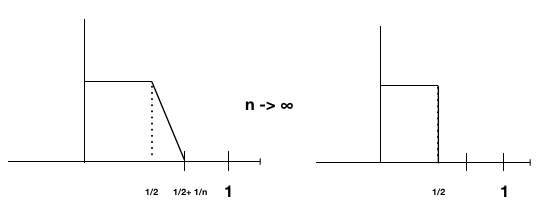
\includegraphics[width=0.5\linewidth]{Screen Shot 2024-01-21 at 10.59.57.png}
    \caption{Una función $C^0[0,1]$ }
    \label{fig:enter-label}
\end{figure}

\underline{Ejemplos}
\begin{enumerate}
    \item $C^0( \Bar{\Omega} ) \text{ con } |f|_{0} = \underset{\Bar{\Omega}}{\max} |f(x)| $
    \item $C^1(\Bar{\Omega} ) \text{ con } |f|_{1} $
    \item $L^2(\Omega)$ por definición   $ = \{ f con  \{ f_n\}  \text{ continua, }  \iint |f_n -f_m|^2 < \infty  \text{ con } f_n \rightarrow f  \text{ y } \iint |f|^2<\infty  \} $
    \item $H^1(\Omega)$
\end{enumerate}

Sea $U\equiv \text{Vecindad de } f \in E  \Rightarrow \{ U \in E \} \supset  \{ g \text{  con  } || g - f || < \epsilon \}$,
definimos un punto de acumulación de $A\subset E$ ,  si $f\in E $ es punto de acumulación de $A$ si 
existe una sucesión $ \{ f_n \} \in A $ con  $f_n\rightarrow f$.

$\Bar{A} = \text{cerradura}  = A \cup \{ \text{puntos de acumulación} \} $


$A \text{ es \underline{ denso } en } E \text{ si } \Bar{A}  = E $


$Q$ es denso en $\mathbb{R}$


$\{ Polinomios\} $ denso en $L^2(\Omega)$


$\{\Bar{\Omega} \text{ compacto denso en } | |_0  \} \subset  C^0(\Omega)$ Stone-Weistrass

 
$E$ de Banach es \underline{separable} si existe un conjunto numerable denso en $E$


$C^0(\Bar{\Omega})$ es separable 


$L^2(\Omega)$ es separable 

Polinomios con coeficientes en $\mathbb{Q}+i\mathbb{Q}$ es separable

\section{Dependencia lineal}

Sea $E$ normado $f_1,..., f_n \in E$ son linealmente dependientes si existen $\lambda_1,...,\lambda_n$ escalares no todos cero
tales que


$\sum\limits_1^n \lambda_i f_i =0 \text{ en } C^0(\Bar{ \Omega}) : \sum\limits \lambda_i f_i(x) =0 \forall x\in  \Bar{ \Omega}$

$L^2(\Bar{\Omega} \Rightarrow \sum\limits \lambda_i f_i(x) = 0 $ \text{ a.e (almost everywhere) }

\begin{lemma}
Si $E$ tiene producto escalar, $f_1,...,f_n$ son linealmente independientes si y solo si
$D=$ matriz.  $D_{ij}= (f_i,f_j)$ es singular 
\end{lemma}

\begin{proof}
"$\Rightarrow$"  Si $\sum\limits_{j=1}^n \lambda_jf_j = 0 $   $\Rightarrow (f_i,\sum\limits_{j=1}^n \lambda_jf_j ) = \sum\limits_{j=1}^n \lambda_j (f_i, f_j ) =  \sum\limits_{j=1}^n  D_{ij} \lambda_j$
Es un sistema lineal de ecuaciones homogeneo, que para que tenga solución distinta de cero su determinante debe ser cero.
\end{proof}

\begin{ejemplo}
    \begin{enumerate}
        \item $L^2[0,1]$  $1,t,t^2,t^3,...,$ son linealmente independientes
        $(t^i, t^j)= \int_0^1 t^i t^j dt = \frac{1}{i+j+1}$

        \[
        D= \left( 
        \begin{array}{ccccc}
            1& \frac{1}{2}& \frac{1}{3}& \cdots& \frac{1}{n} \\
            \vdots & & & &\\
            \frac{1}{n} &&& & \frac{1}{2n+1}
        \end{array}
        \right)
        \]
    Se puede ver que su determinate es cero    
    \item $L^2[0,\pi]$  $1,\cos x, \cos 2 x, ..., \cos n x$ son linealmente independientes. $D$ es diagonal,
    tambien $1,\sin x, \sin 2 x,..., \sin n x $ 
    \item $L^2 [0,2\pi]$  $1,\cos x, \sin x, \cos 2x, \sin 2x,..., \cos nx, \sin nx $ son linealmente independientes $D$ diagonal
    \item $L^2_{\mathbb{C}}[0,2 \pi]$   $e^{ijx}, j=-N,...,M$
    
    \end{enumerate}
    
\end{ejemplo}

\begin{definition}
$f \perp g  \Leftrightarrow (f,g) = 0$ 
\end{definition}

\begin{definition}
$\underset{f_i\neq 0}{\{f_1,...,f_n\}}\in \underset{(,)}{E}$ son ortogonales si $(f_i,f_j) = 0 \; i\neq j $ y son \underline{ortonormales} si $(f_i,f_j) = \delta_{ij}$ 
\end{definition}

\begin{theorem}
Sean $\phi_1,...,\phi_n,...$ ortonormales en $E$ con $(,)$
sea $U\in E$ y $ U_n = \sum\limits_1^n (U,\varphi_j) \varphi_j = \sum\limits_1^n \alpha_j \varphi_j$
$\alpha_j$ se llaman los coeficientes de Fourier de $U: L^2_{\mathbb{C}} [0,\pi ] , \phi $

Si $\varphi_j = \frac{ e^{ijx} } {\sqrt{2\pi}}$
\[
(\varphi_k,\varphi_j)= \int_0^{2\pi} \frac{e^{ikx}}{\sqrt{ 2\pi}} \frac{e^{-ijx}}{\sqrt{ 2\pi}} dx= \frac{1}{2\pi} \int_0^{2\pi} e^{i(k-j)}x dx = \delta_{ij}
\]

\[
\alpha_j=\frac{1}{\sqrt{2 \pi}} \int_0^{2\pi} U(x) e^{-ijx} dx
\]

$\Rightarrow$

\begin{enumerate}
    \item $\Vert U-U_n \Vert \leq \Vert U - \sum\limits_1^n \lambda_j \varphi_j \Vert \;\; \forall \;\; \lambda_1,\ldots, \lambda_n$ con igualdad solo si $\lambda_j= \alpha_j$

\begin{figure}
    \centering
    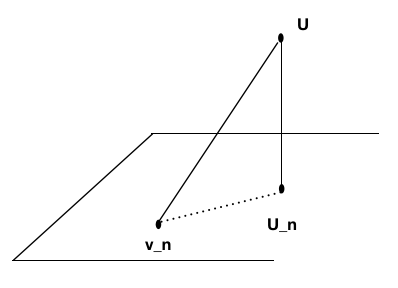
\includegraphics[width=0.5\linewidth]{Fig_2.png}
    \caption{Proyección ortogonal de U sobre $E_n= < \varphi_1, \ldots, \varphi_n >$ }
    \label{fig:2}
\end{figure}

\item Desigualdad de Bessel  
\[
\sum_1^{n} |\alpha_j|^2 \leq \Vert U \Vert^2 
\]
y si $E$ es de Hilbert $\Rightarrow$  $\sum\limits_1^n \alpha_j \varphi_j$ converge en $E$ 

\end{enumerate}

\end{theorem}


\end{document}